\setcounter{equation}{0}
\chapter{Introduction}
  Throughout human history technological innovation has redefined our experience in the world, changing the way we interact with each other and the perception of the distances that separate us. Communication is basic need for anyone; however, our expectations on what communicating means has transformed through time. Most recently, from the beginning of the new millennium we require fast, long reach and high capacity telecommunication systems, like  the telephone network or the internet. This are not simple requirements, consider that just under 250 years ago the United States Postal Services was established to bring a way of sending and receiving information through a robust network throughout North America, which was a great innovation at the time, but it does not come close to fulfill the requirements that seem natural to us today. Our current communication needs are in some ways more similar to the mailing system than to a phone network in the beginning of the 19th century. We expect to send and receive packets of any size, to a location as convenient as possible, with reliable service and with little hassle to the user. A phone network from the beginning of the 19th century was nothing close to this, usually with single phone for large areas. It was connected by operators that required information from the user and had poor coverage with low reliability.

Today we take for granted the technology developed to satisfy our need to communicate over a reliable and robust network.  It is common practice for most of us to connect with family members or friends that may be anywhere around the world or request information from any server in the world. Just two decades ago it wasn't possible to depend so reliably on the communications networks due to low capacity, lack of redundancies and inefficient routing schemes that added latency to the network~\cite{HistoryCommunication}. As powerful as our current networks might be, it is the human way to find higher and more complex requirements for the way we communicate. When the first consumer deployment of 3G in 2001 was implemented most consumer analytic professionals questioned the idea of offering such a large capacity to consumers~\cite{HistoryCommunication}. At the time there was no service that used the full capacity of the bandwidth offered. Now we know that you just have to give the tools to the public and use scenarios will show up as did Meme sharing or video streaming. 
        

Current networks can handle heavy loads but in the future the need of low latency communication ( for self-driving cars or remote surgeries), the Internet of Things (IoT), high quality video streaming and others will require creative solutions to the current limits of communication systems.  New technology will be deployed in the network, improving its capacity, but there is also a need to extract as much use from older networks to maintain there current coverage and reduce costs. Coherent Optical telecommunications gives a path forward that improves the network as whole, improving the current operating network and pushing the limits for the future transparent network~\cite{ModForm,NetGenTransp}.

\section{General Objective \& Motivation}	
In coherent optical communication the effects of dispersion and attenuation can now be compensated for. However, the noise that arises from the interaction between the optical power and the fibers optical Kerr effect limit the transmission length of the system~\cite{NLPNinCFO}. The noise sources that arise from this interaction are known as nonlinear interference noise. The aim of this thesis is to study the effects of nonlinear noise in a coherent optical communication system and suggest a \textit{nonparameter digital signal processing detection scheme} enabled by machine learning. Two communication links are built, a \textit{long-haul} and a \textit{dense wavelength division multiplexed} system, to detect nonlinear interference noise. Each communication link architecture is used to test if the suggested digital singal processing scheme improves the transmission distance of the signal compered to a  traditional scheme.    


Bringing together machine learning and optical communications has been on surge for the past decade and has been implemented in performance monitoring~\cite{shen2010optical,jargon2008optical}, modulation format identification~\cite{khan2012modulation} and amplitude/phase noise characterization~\cite{zibar2015application}. This techniques improve the performance of the system and extends the operational capacity. Increasing the transmission length of the optical system allows a further reach simplifying the deployment of the network, and reducing the need of re-transmitter. Given that the most expensive part of deployment is digging and laying optical fiber it is necessary to reduce the deployment complexity and cost. Getting more use from older network segments helps improve coverage as well, resources can be allocated to reach more people instead of having to lay again the same network segments. The current bottle neck in a fiber link is the presence of nonlinear noise~\cite{NLPNDSP}, machine learning could be a way to mitigate nonlinear noise without needing any information on the physical state of the fiber system~\cite{Nonparameter}. This is a relatively novel idea that has been implemented in References~\cite{Nonparameter,zibar2015application} and others. Our approach implements algorithms that have been improved over time and now enable more efficient and robust predictions.  






 



\section{Optical Telecommunications}

Transporting information requires a protocol that standardizes a measurement of a physical event. Through time there have been many information links used to communicate at a distance from a smoke signal or a telegraph up to the telephone. All these have revolutionized our way of communicating and the reach at which we can expect to get an immediate response. Optical communication is the field interested in studying the implementation of communication systems using light as an information carrier. The beginning of Optical communication by this definition could be traced back to the Greeks in 1084~B.C where its said that a 500-km-long line of fire beacons was built to convey urgent messages, like the fall of Troy~\cite{HistoryCommunication}. In the framework we understand optical communication now, a first proposal of a Fiber-Optic Communication was done by Jun-ichi Nishizawa in 1963 at Tohoku University~\cite{ProposeFiberCom}. This type of lightwave system uses optical fiber to contain a light pulse guiding it to a receiver, where it is detected  and decoded into a digital signal containing information like voice message or video.

Today fiber-optic communication is the most prominent technology in long-haul communication, enabling the vision of a global society thanks to its effective reduction of immediate communication length. Fiber optics has also had a large implementation in the metro networks in the paste decade, due to improvements in fibers made out of polymers, reducing the cost of deployment \cite{AccesFiber}. When we place a call or use the internet, we expect a fast, reliable and robust coverage. These requirements set high constraints into the technology  development. Not all communication needs can be satisfied with the same technology.

 Currently, a combination of electrical and optical systems are used depending on the requirements given, each scheme has benefits an drawbacks. For long haul communications it is necessary to have a system that can be implemented over hundreds of kilometers, with high capacity and low latency, making fiber optics an ideal technology. Today's optical communications systems can fulfill these requirements but it has taken a lot of effort to develop and perfect a reliable communication link~\cite{COChistory}.   

\subsection{Brief History of Optical Communication}

A more contemporaneous start to \textit{optical communications} would be the invention of the optical semaphore telegraph in the 1790s by C. Chappe~\cite{opticalsemaphore}. However, it took one more century for a new development in the field, in 1880s A. Bell created the Photophone an optical telephone system that never saw much use~\cite{opticalsemaphore,HistoryCommunication}. The 1960 marked a true revolution in optical communication thanks to the invention of the \textit{laser} and \textit{glass fiber}~\cite{ramaswami2009optical}. C. K. Koa, G. Hockman and J. Nishizawa  where among the first to notice the potential of this new technologies~\cite{kao1966dielectric,ProposeFiberCom}, they realized that the attenuation in a fiber could be reduced to a usable value of 20~dB/km by decreasing the impurities in the glass fiber. At this time the attenuation was approximately 1000~dB/km in a usual fiber.\textit{ Corning Glass Works} was able to manufacture the worlds first low-loss single mode fiber operating at 633~nm with an attenuation of 20~dB/km in the 1970 making it commercially available by 1975~\cite{opticalsemaphore,HistoryCommunication}. The technological developments  achieved through the history of Optical Communications  can been divided into four generations. Distinguishing from each generation the operating wavelength, data rate and transmission distance.

In the starts of 1975 the commercially available communication system was a multimode fiber with a 800~nm GaAs semiconductor laser. The systems main limitations was the high fiber loss, intermode and intramode dispersion~\cite{OFCNetwork}.  Giving it a performance of 45~Mbit/s for a transmission distance of 10~km without repeaters. A set of improvements  would be carried out in the next five years that tripled the data rate; thus, naming this first implementation a\emph{ first generation} link.~\cite{COChistory} 

Improvements done in 1980 allowed further reach and higher bit rate operation. By changing the operating wavelength and breakthroughs in glass fiber manufacturing substantial improvements to the technology where archived ~\cite{COChistory,Sharma2013ARO}. Marking the start of the \emph{second generation} link, which had a new  InGaAsP semiconductor laser operating at 1330~nm with a low loss -at the time- 1dB/km single mode fiber. Second generation optical communication systems could reach a data rate of 1.7~Gb/s with a transmission distance of 50~km without repeaters ~\cite{ModForm,Sharma2013ARO}. A significant improvement over the first generation; however, the fiber losses where still high and no dispersion management had been implemented yet. 

At the beginning of the 1990 a solution was found to mitigate the fiber losses and have the minimum dispersion coefficient around the operating wavelength. The development of dispersion shifted fibers~\cite{COChistory} enabled deploying longer fibers without presenting dispersive effects.  The new communication system operated with a low loss single mode fiber 0.2~dB/km at 1550~nm. The two main breakthroughs in this \emph{third generation} system was the shift to an operating wavelength with minimum attenuation and the improvement in the core-cladding fiber design such that the chromatic dispersion is minimum at the 1550~nm wavelength region. This system achieved a data rate of 2.5~Gbit/s at a
transmission distance of 100 km without repeaters~\cite{ModForm,Sharma2013ARO}. Multiplexing and transparent amplification  where the last two key technologies needed for a robust communication system.

The last three decades have brought a fleet of improvements, three different types of information multiplexing, the invention of transparent amplification and higher order modulation formats, enabling  109~Tbit/s performance with further reach without repeaters. \textit{Wave division multiplexing} (WDM), \textit{polarization division multiplexing} (PDM) and \textit{time division multiplexing} (TDM)~\cite{kikuchi2008coherent,ModForm,Sharma2013ARO} have helped extract as much capacity as possible from different communication systems. The \textit{erbium dope fiber amplifier} (EDFA) gave way to longer transmission range without repeaters and DFB lasers with stable phase coherence enabled the implementation of higher order modulation formats. \emph{Fourth generation} optical communication system are defined by use of this technologies. Currently, fourth generation systems are still operational and Telecom operators are interested in extending the life span of this systems as a cost effective update.    

\subsection{Current Outlook in Optical Communications}


The lightwave systems currently deployed are referred to as Intensity Modulation with Direct Detection (IM/DD). An alternative to IM/DD is to transmit information by modulating the frequency, amplitude or  phase of the optical carrier. Detection of the transmitted signal is done by a scheme known as \textit{coherent detection} that allows the extraction of all the signals information. Phase coherence with the optical carrier plays an important role in Higher-Order Modulation (HOM) format links, also known as \textit{coherent lightwave systems}. These systems fall into the field known as  \textit{Coherent Optical Communications}, that has been studied extensively since the 1980. Its deployment was slow at the time due to limitations on amplification and cost effective improvements in IM/DD systems~\cite{FiberAgrawal,NetGenTransp}.

 Coherent optical receivers follow a heterodyne detection scheme where a \textit{local oscillator} (LO) is required to detect the incoming signal.
When the LO and the transmitted signal are mixed, a beat frequency equal to the difference between the two frequencies is created. By adjusting the local oscillator frequency, the beat frequency retrieved could be the signal that was modulated on top of the optical carrier. These detection arrangement makes the receivers require more power and physical components. At the time IM/DD receivers where cheaper to run and manufacture making them more widely deployed. In current networks IM/DD system are reaching their limit~\cite{COChistory}, this has brought new interest to coherent systems, thanks to the possibility of improving already deployed links and giving space to create new solutions for future demands. Currently, the main objective of coherent optical communications is exploiting Photonics to engineer the next generation transparent network. However, a main limitation is phase noise distorting the signal while it propagates through the fiber making noise compensation a vital part for a high quality link~\cite{behrens2010nonlinear}.

\section{ Modulation Formats }
 
 
 A HOM format is a scheme to standardize information for a correct representation of a signal and extract a bit stream from a physical measurement. In optical communication the amplitude and phase of a DFB \textit{continuous wave} laser is modulated to encode information in them, this information can be later decoded at the receiver side by heterodyne detection. A single detection of a combination of phase and amplitude components is denominate a \textit{symbol}. A set of M unique symbol can be mapped to unique bit sequences of m bit long. A graphical representation of the modulation  of  optical carrier is shown in Figure~\ref{fig:AmPm} which depicts the basic transformations that can be done to the carrier. In digital communication  \textit{amplitude} and \textit{phase} are referred to as the \textit{in-phase} and \textit{quadrature} components or IQ components. It is usual to represent the transmission signal in phase diagram as shown in Figure~\ref{fig:QAMcons} where you can represent each symbol by its IQ components also known as a constellation point when represented in a phase diagram. When the carrier signal is  \textit{amplitude modulation} (AM) or \textit{phase modulated} (PM) the transformation under gone in the phase diagram is just a translation or rotation, as shown in the top left of Figure~\ref{fig:QAMcons}.
 
  \begin{figure}[h]
 \centering
 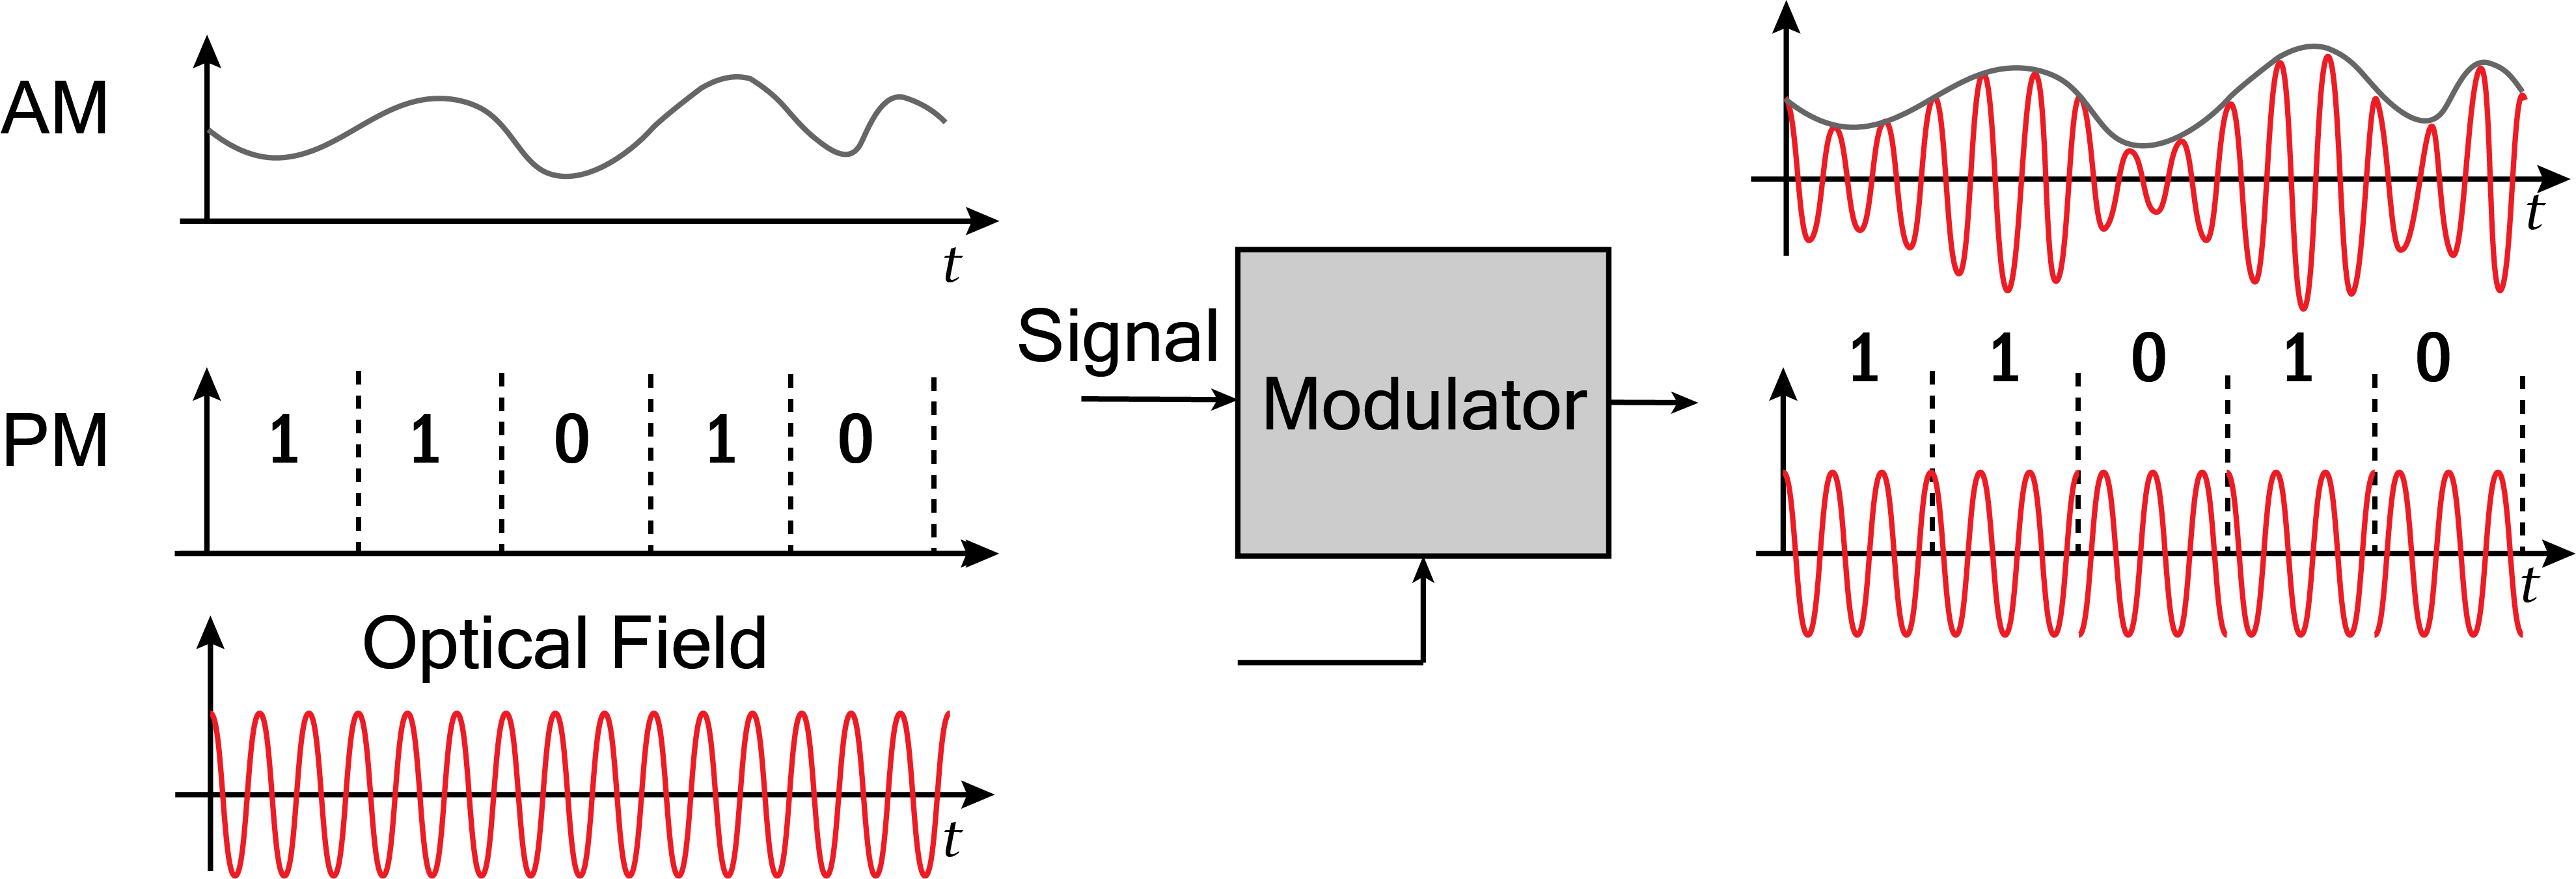
\includegraphics[width=0.8\linewidth]{modulationShow.png}
 \caption{Amplitude modulation and phase modulation can be implemented to transmit information over a optical field. In this figure a visual representation on how information can be imprinted to a carrier signal is shown. }
 \label{fig:AmPm}
 \end{figure}
 With this two basic transformations, an array of modulation formats are possible. A modulation format is in general a scheme to determine a set of equidistant points of unique IQ component that each represents a unique bit sequence, also called a constellation. The most simple case is the \textit{binary phase shift keying} (BPSK) that consists of two unique constellation points, determining how to classify a detected symbol is simple if it falls to the left of the y-axis the symbol is a 1 or if it falls to the right the symbol is a 0. Thus a simple decision region dividing in half the phase diagram would suffice to accurately classify the detected symbols.
 
  An extension to phase modulated BPSK can be achieved with a clear signal, higher resolution on the receiver and increasing the amount of constellation points. Modulation formats like \textit{quadrature phase shift keying} (QPSK) or \textit{eight constellation point phase shift keying} (8PSK) are extension on BPSK as can be seen from the constellation diagram (observe Figure~\ref{fig:QAMcons}). To transmit more bits per symbol, it is useful to have a compact constellation diagram. Thus, using both AM and PM is a logical next step to modulate the carrier signal.
 
 \begin{figure}[h]
\centering
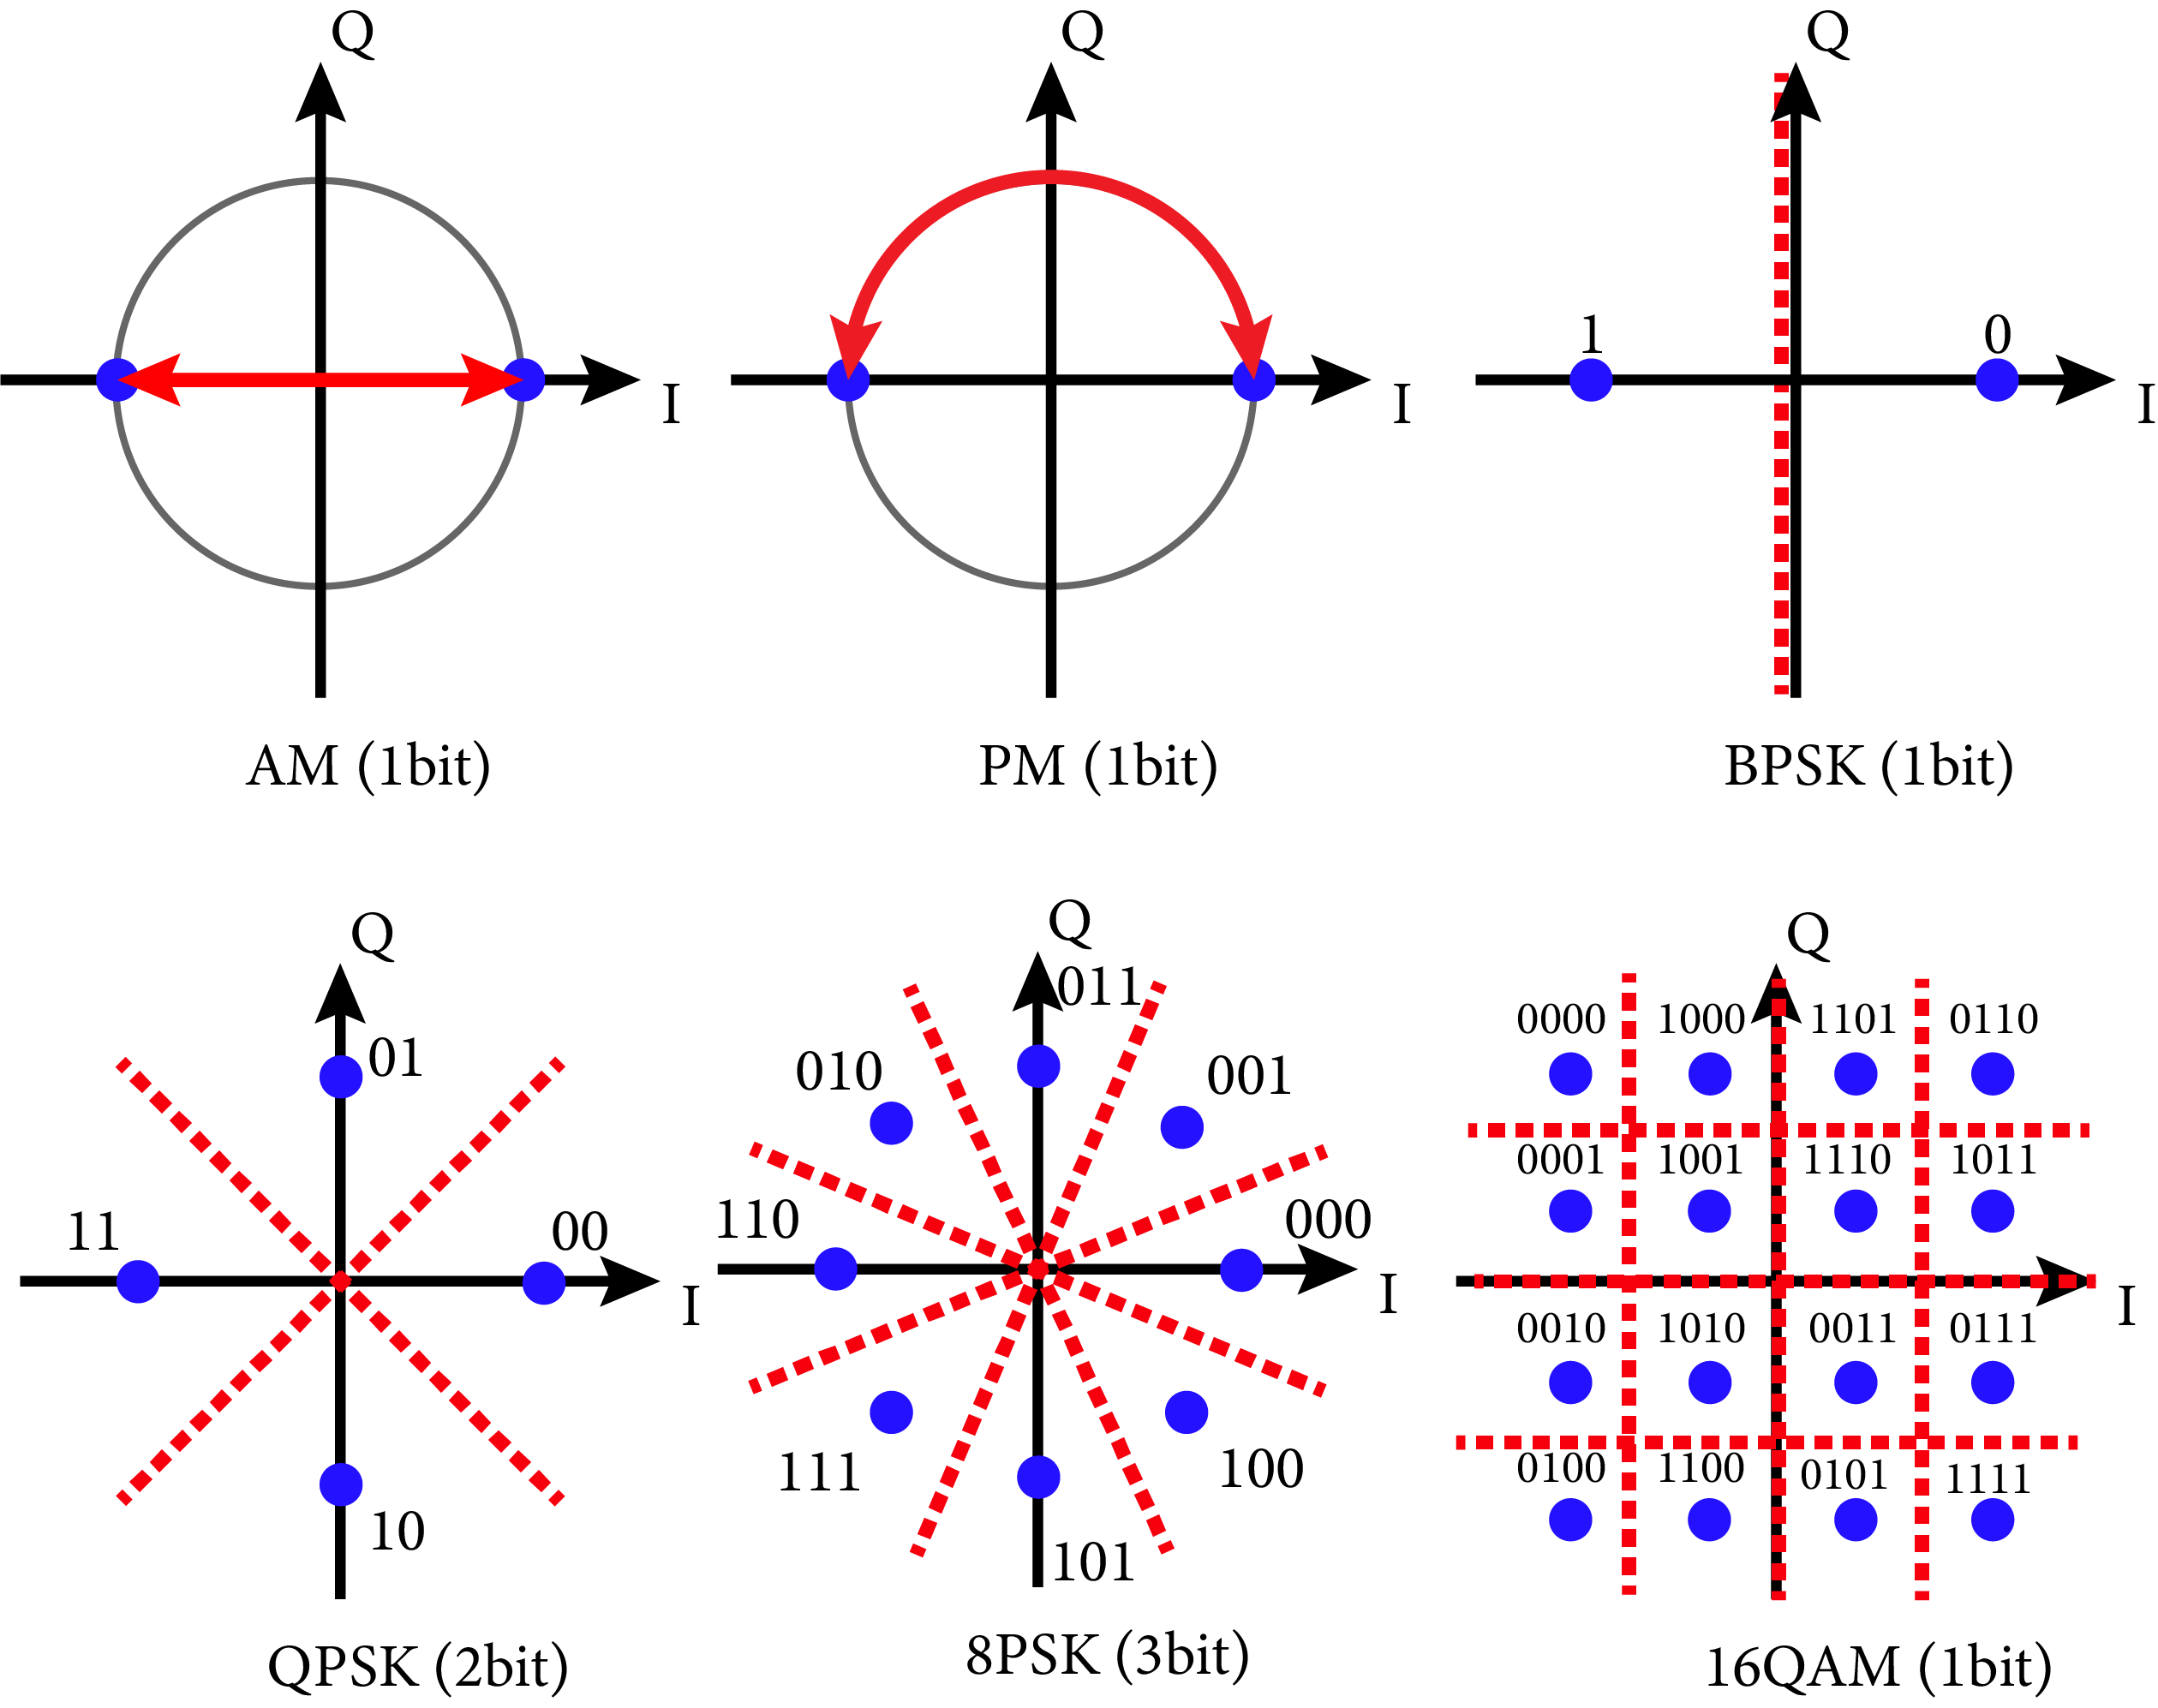
\includegraphics[width=0.7\linewidth]{QAMcons.png}
\caption{A phase diagram can be used to represent the changes in the state of detected signal. A HOM  implement more complex constellations architectures to transport more information per symbol.     }
\label{fig:QAMcons}
\end{figure}

A widely implemented modulation format in modern telecommunications is \textit{Quadrature Amplitude Modulation} (QAM), a technique in which two carriers shifted in phase by 90 degrees are modulated and combined. Due to this phase difference the carriers are in quadrature, giving the modulation format its name~\cite{benedetto1999principles}. This technique allows a communication system to reach higher data rates within the same bandwidth and higher spectral capacity~\cite{webb1994modern}. The number of bits \emph{m} needed to decode each symbol  is related to the number of symbols $M$ or constellation points that represent all bit unique combinations as $M=2^{m}$~\cite{paik1994mode}.  A representation of a 16QAM square constellation is shown in the bottom right of Figure~\ref{fig:QAMcons}, the corresponding constellation point and decode 4~bit message are displayed for each symbol. The quality of the link relies on having little noise, such that the transmitted symbol can be detected with its original phase and intensity. Making noise mitigation a necessary component for robust systems. 
 
 
  
 \section{Optical Noise}
  
Photonics gives a framework to describe and engineer a communications link that can have high capacity, low latency and long-distance coverage. A wide range of creative solutions are required to counter impairments that arise from the light-matter interaction between the light pulse and the fiber cable. When noise is present in a channel, it deteriorates the quality of the signal. The quality of the signal can be quantified  by the Optical Signal to Noise Ratio (OSNR). Information is imparted onto a light pulse by modulating its physical properties within a predetermined scale or protocol like a HOM. The main purpose of a communication link is to transmit symbols that can be decoded into bits, the amount of errors encountered in a bit stream is known as \textit{bit error rate} (BER). It is worth mentioning that the \textit{symbol error rate} (SER) does not have to be the same as BER, depending on the modulation format and the \textit{forward error correction} (FEC) there can be significant difference reducing the actual amount of mistakes made~\cite{benedetto1999principles}. 


When light propagates through a medium it can suffer a change in speed depending on its wavelength, this effect is known as \textit{chromatic dispersion} (CD) or \textit{group velocity dispersion} (GVD). A pulse of light contains multiple wavelengths  rather then a single frequency. Thus, when the pulse acquires CD it stretches in time, affecting the timing of the link corrupting the information carried.  Dispersion is not the only noise source in a fiber link, the inline optical amplifiers that counter the fiber attenuation produces \textit{amplified spontaneous emission} (ASE) noise which is added to the signal as \textit{additive white gaussian noise} (AWGN), reducing the OSNR. Amplifiers contribute to other types of noise indirectly, like the noise produced by intense light propagating through a medium~\cite{FiberAgrawal}.

The architecture of the detector can also add noise  to the received signal depending on the resolution of a heterodyne detection with a large offset between the incoming signal and the LO, known as the \textit{carrier frequency ofset} (CFO). Linear sources of noise arise primarily from the response of the dielectric -the silica optical fiber- to low intensity light propagating through it. 

In the regime of low intensity light a transparent medium is represented by its refractive index. The electrical susceptibility of the medium is connected to its optical response, the linear or first order response is connected to the refractive index. The higher order or nonlinear response of the susceptibility has a small contribution to the total interaction at low intensity. The higher order susceptibility only has a significant contribution in the presence of an intense electromagnetic field like an intense laser or tightly confined light, as presented in the waveguide geometry of a fiber. Some part of these noise sources can be mitigated using \textit{digital signal processing} (DSP), clever exploitation of physical phenomena on pre/post-compensation extending the throughput of the link~\cite{agrawalapplications}.     
      


A critical limiting factor is \textit{nonlinear interference Noise} (NLIN) produced by the interaction between the signal and the ASE noise via the higher order response of the electrical susceptibility. Compensating for nonlinear effects is possible, using pre-compensation or DSP~\cite{NLPNinCFO}. However, the main adversity to these techniques is the requirement on knowing the physical sate of the link, which is possible in a point-to-point link but it is not practical for a deploying a dynamic optical network. 

Nonlinear noise set the limit for the maximum amount of information transmitted over a set distance of  an optical communication link~\cite{PrincBorn}. Restriction in optical power help reduce nonlinear noise, but high power is also necessary in HOM to obtain the necessary OSNR, limiting how low the power should be set. Noise mitigation becomes then interesting to retrieve an accurate representation of the link that permits computing decision regions for the transmitted symbols based on the links configuration. However, having a complete physical representation of the link is an impairment in real deployment, since there must be some tolerance in the real specifications and its cumbersome to keep count of system length, type of fiber etc. Nonparameter noise mitigation is a novel solution to mitigate nonlinear noise in a system where the physical attributes are unknown, the detection scheme would produce the most reliable decision regions based on the noisy signal~\cite{NLPNmPSK}.  
          

 
 
 \subsection{Optical Noise in a QAM Channel}

In a QAM channel NLIN is imparted as a phase shift to each symbol. Since the HOM classifies each symbol based on its phase (Figure~\ref{fig:QAMcons}) a phase shift could change the classification of the symbol.
The reduction of the OSNR due to the noise produced by the linear susceptibility is visualized  in Figure~\ref{fig:LinerNoise}, where the different sources of noise previously mentioned are shown for the case of a square 16QAM constellation. Mitigation techniques can improve the quality of the signal in the case of CFO, but improving the OSNR is not possible due to the non-stochastic nature of linear noise. 


  \begin{figure}[h!]
 \centering
 \subfloat[Standard OSNR  25dB ]{\label{fig:NoNoise}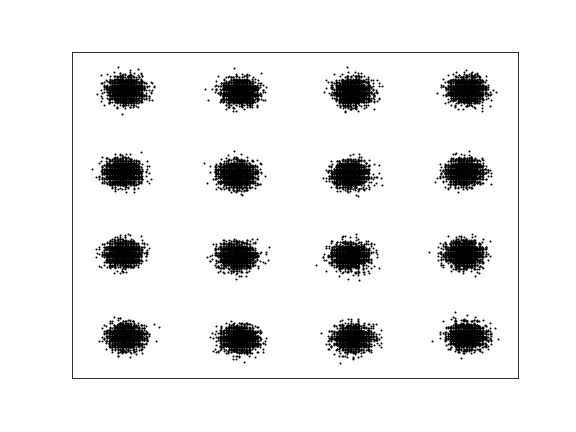
\includegraphics[width=0.3\textwidth]{NONoise.png}}
\subfloat[Low OSNR 15dB]{\label{fig:AWGNoise}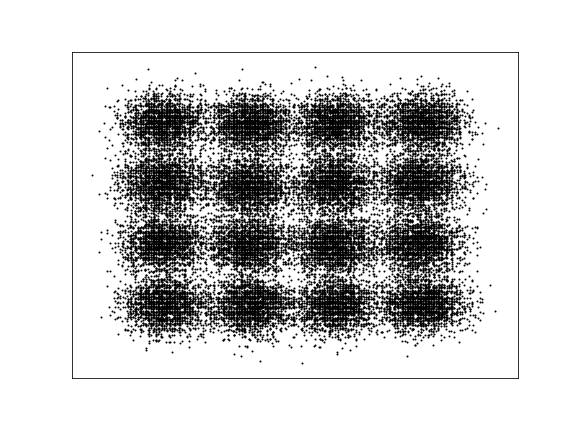
\includegraphics[width=0.3\textwidth]{AWGNoise.png}}
  \subfloat[CFO phase noise]{ \label{fig:LONoise}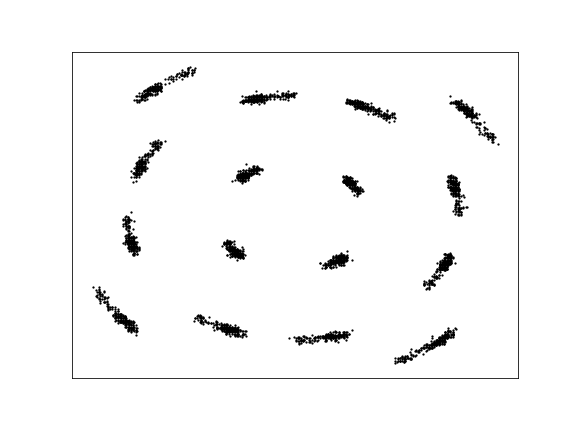
\includegraphics[width=0.3\textwidth]{LONoise.png}} 
 \caption{Square 16QAM constellation comparison between different types of linear noise. }
 \label{fig:LinerNoise}
\end{figure}
 In the presence of an intense light source, as is needed in QAM, nonlinear noise distorts the signal and hampers the transmission distance. Nonlinear effects also alter the constellation of a QAM link, an example of this distortions is shown in Figure~\ref{fig:NLPNcons}.  Nonlinear noise has the advantage of being stochastic source of noise, such that a probability distribution could be extracted from the noise~\cite{Zibar:12}. From Figure~\ref{fig:NLPNcons} it is noticeable that the decision region for each symbol has to be more complex than in the case of Figure~\ref{fig:LinerNoise}. 


\begin{figure}[h!]
 \centering
\subfloat[Gordon-Mollenauer effect ]{\label{fig:NLPNoise}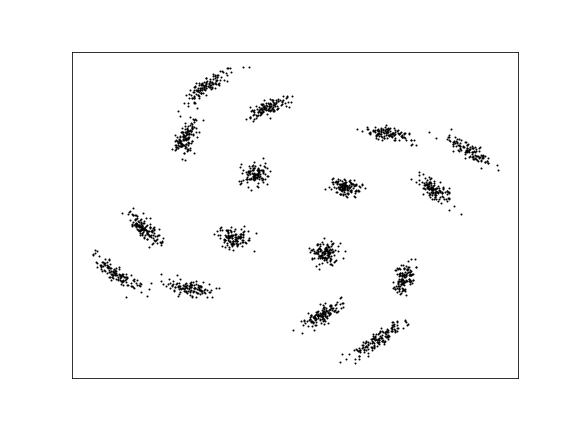
\includegraphics[width=0.45\textwidth]{NLPNoise.png}}
  \qquad
  \subfloat[Cross phase modulation]{ \label{fig:WDMNoise}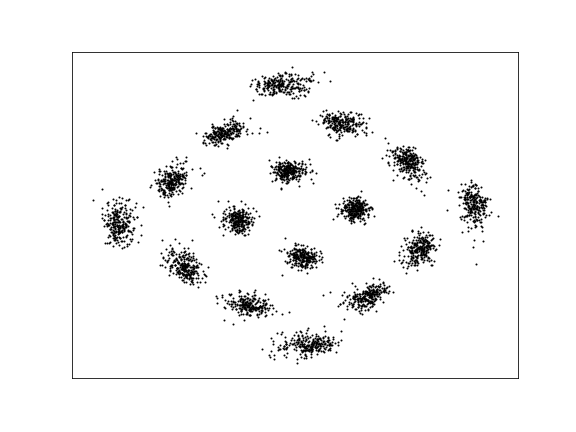
\includegraphics[width=0.45\textwidth]{MUXNonlinearNoise.png}} 
 \caption{16QAM constellation comparison between different types of Nonlinear Noise }
 \label{fig:NLPNcons}
\end{figure}
 Complicated decision regions have been implemented through DSP and nonlinear back propagation~\cite{NLPNDSP} showing improvements on a known system. An other approach is being done through \textit{machine learning} which show unique advantages~\cite{Nonparameter,Zibar:12} by making accurate predictions with out the need of back propagation or heavy numerical analysis. A more detailed description of the DSP and machine learning will be presented later on in this report.

% 	
\section{Machine Learning}
%
Learning has been a fundamental ability for humans throughout time, observing our surrounding, using tools and developing technological advancements are only possible due to the ability to remember previous  experiences to make prediction of the future. Since 1957 with the development of more powerful computers and more sophisticated software, the notion that a machine could \emph{learn from data} in comparable way as humans\emph{ learn from experience} has captivated many~\cite{kaplan2019siri}. As currently defined Artificial Intelligence (AI) uses a computer to perform cognitive tasks; such as, perception, learning, reasoning or other similar abilities. A branch of AI is \textit{machine learning} (ML), based on the idea that patterns and trends in a given data set can be learned through some algorithm. From the learned structures a decision or prediction can be made for some other data set in the system of interest~\cite{marsland2014machine}.

\begin{figure}[h!]
 \centering
\subfloat[Random Forest ]{\label{fig:ForeML}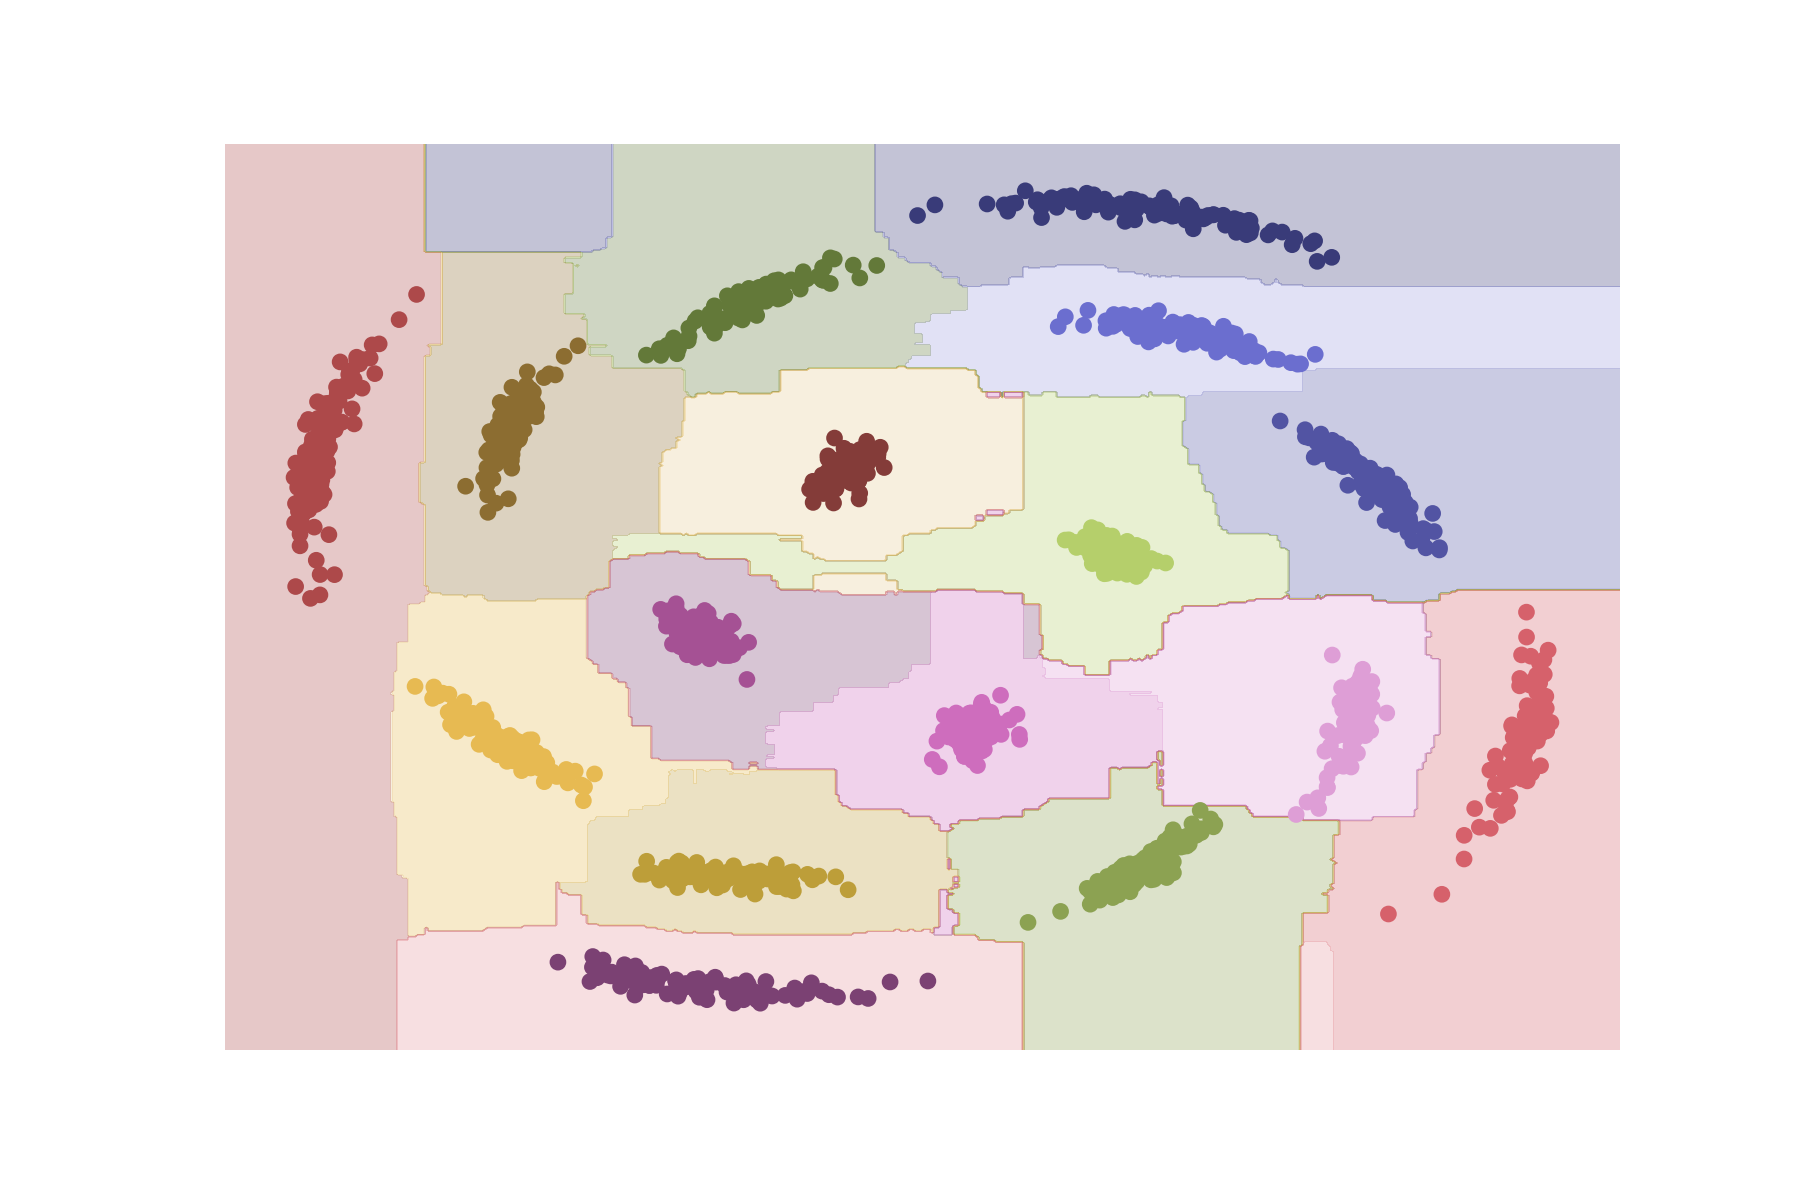
\includegraphics[width=0.46\textwidth]{ForeN26L80X.png}}
  \qquad
  \subfloat[Support Vector Machine]{ \label{fig:SVCML}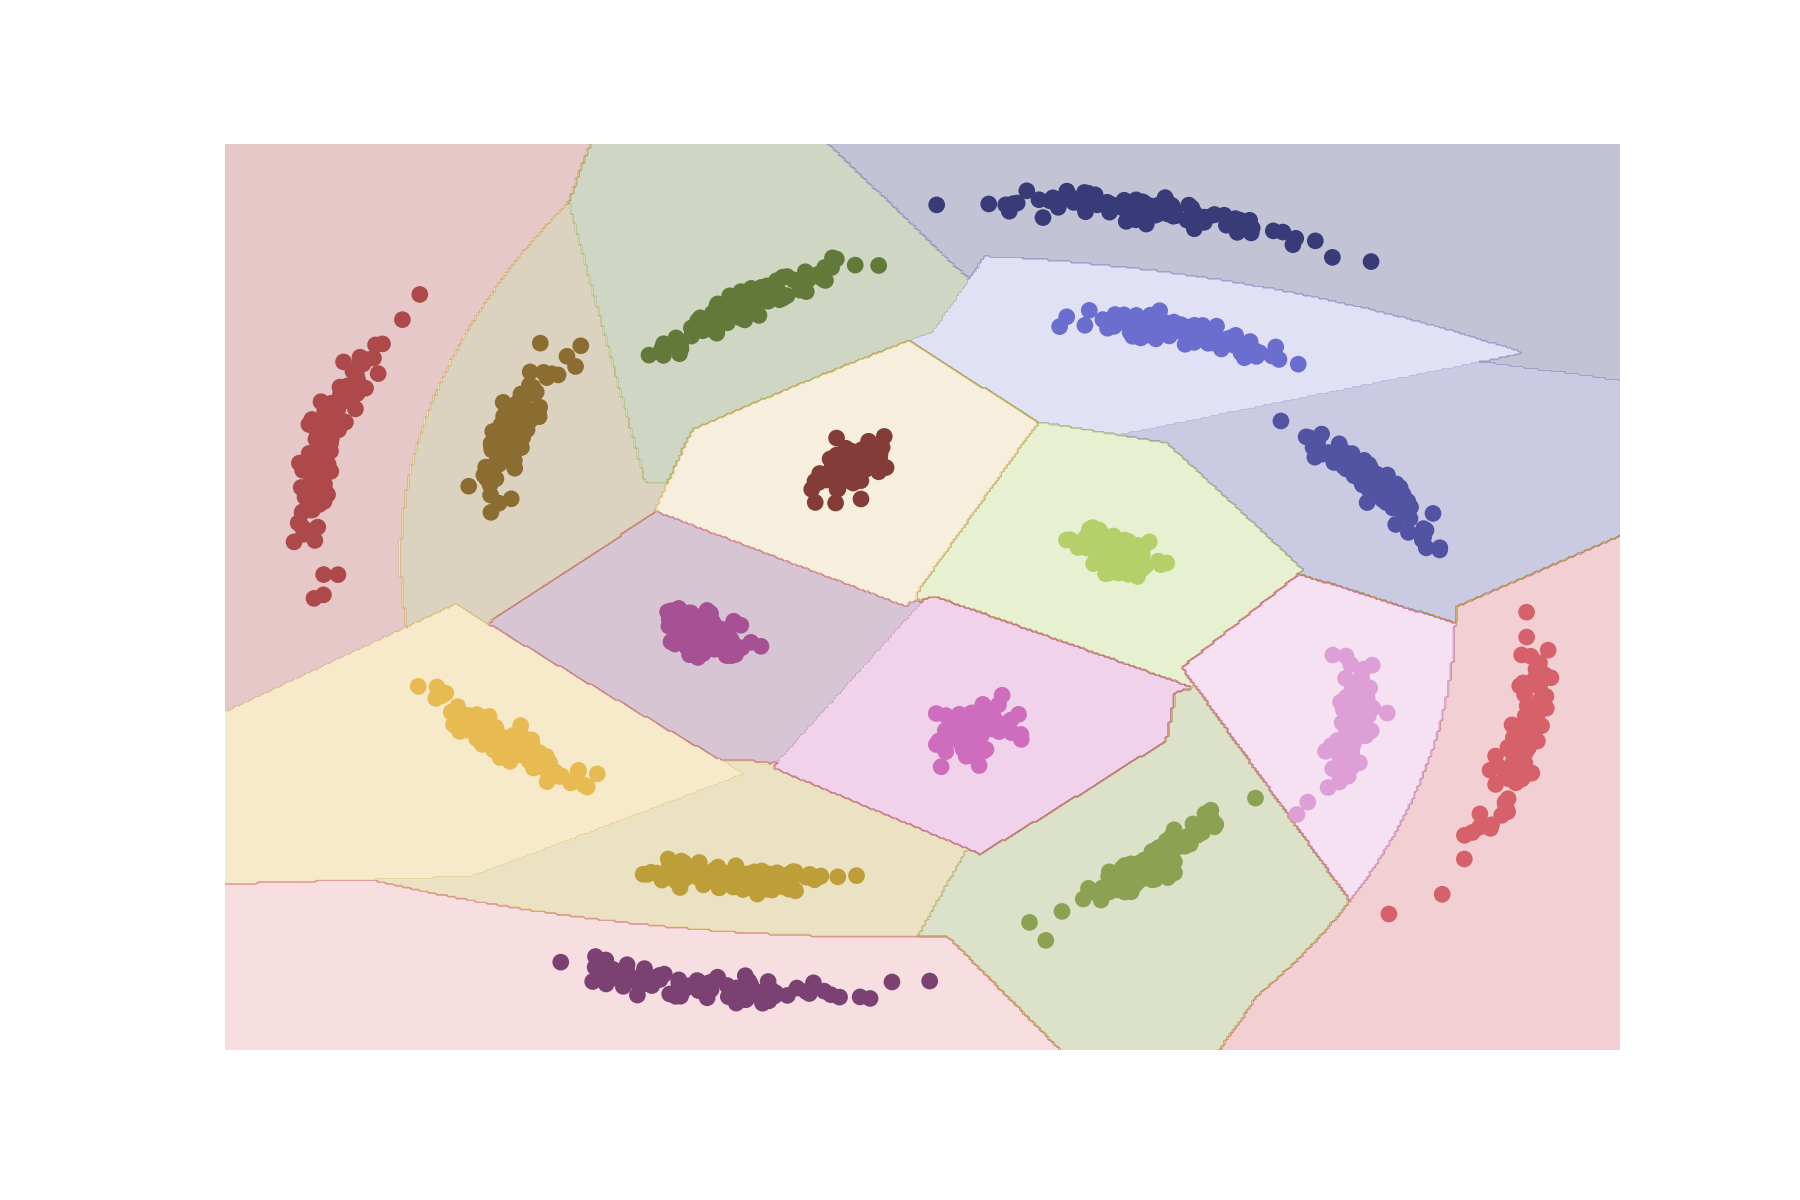
\includegraphics[width=0.46\textwidth]{SVCN26L80X.png}} 
 \caption{Machine learning determined decision regions for  16QAM constellation with NLIN acquired from 26 segments of 80 kilometer fiber.  }
 \label{fig:MLcons}
\end{figure}

Machine learning is offering a different perspective to problems that traditionally have been solved with complicated numerical models. The term nonparameter detection schemes comes from the idea that ML can suggest decision regions without needing any information on the current state of the link. Thus, ML can be a tool to work around imperfections in a fiber or as our main interest mitigate nonlinear noise sources. In Figure~\ref{fig:MLcons} two different algorithms are implemented to learn the best decision regions for a noisy constellation. Notice how this two ML algorithms perform differently for the same dataset due to their individual learning approach. Our interest is using this algorithms to extend the distance of transmission by improving their prediction capability with noisy signals.   





 



\section{Thesis organization}

This thesis is divided into six chapters that cover the physical description of the system, the digital processing algorithms used and the simulation of the system. In the next chapter the physical layer will be discussed, describing the signal detection, modulation  and the light-matter interaction undergone by the propagating signal in the fiber cable. In Chapter~\ref{ch:DSP} the ML algorithms and a analytically derived algorithm are introduced. After this the simulation of the two communication links and the retrieved data will be presented in Chapter~\ref{ch:simu}. To conclude this report the results will be discussed in Chapter~\ref{ch:simu}, with final remarks and conclusion in Chapter~\ref{ch:con}.  


